% !TEX root
\documentclass[12pt, headinclude=true]{scrartcl}

\usepackage{lmodern}
\usepackage{babel} 

\usepackage{graphicx}
\usepackage{enumerate}

\usepackage{amssymb}
\usepackage{amsmath}
\usepackage{amsthm}
\usepackage{dsfont}
\usepackage{bm}
\usepackage{algorithm}

\usepackage{subfig}
\usepackage{wrapfig}

\usepackage{todonotes}

\usepackage{hyperref}
\hypersetup{
	colorlinks   = true,
 urlcolor     = blue,
 linkcolor    = blue,
 citecolor   = blue
}
\usepackage[noabbrev, capitalize,nameinlink]{cleveref}
\usepackage[round, comma]{natbib}

% \input{latex_templates/layout.tex}
\input{latex_templates/microtype.tex}
\input{latex_templates/theorems.tex} 

\input{latex_shortcuts/math.tex}
\input{latex_shortcuts/stats.tex}
\input{latex_shortcuts/tex.tex} 
 

%------------------------------------------------------------------------------%

\title{Nonparametric Pieced-Together Copula Density Estimation}
\author{Thibault Vatter\\ University of Applied Sciences Western Switzerland}


\begin{document}

\maketitle

\section{Idea}

Let $(U,V)$ be an absolutely continuous random vector with standard uniform margins, and assume that one is interested in estimating its density $c$, called a copula density, based on a random sample $(U_i,V_i)_{i=1}^n$.
Fix a threshold $q_n \downarrow 0$ and write $Q_n=[1 - q_n,1]^2$ for the tail region. In this note, we propose to estimate $c$ by piecing together a bulk estimator on $Q_n^c=[0,1]^2 \setminus Q_n$ and a tail estimator on $Q_n$.

For the bulk, we use the estimator of \citet{geenens2017probit}.
Define the probit-transformed vector $(X,Y)=(\Phi^{-1}(U),\Phi^{-1}(V))$, estimate its density using a Gaussian kernel, and back-transform the resulting density estimator to $[0,1]^2$, that is
\begin{align*}
  \hat c_{B}(u,v)
  =
  \frac{
    \hat f(\Phi^{-1}(u),\Phi^{-1}(v))
  }{
    \phi(\Phi^{-1}(u))\phi(\Phi^{-1}(v))
  },
\end{align*}
where
\begin{align*}
  \hat f(x,y)
  =
  \frac{1}{n b_n^2}
  \sum_{i=1}^n
  K_B\left(
    \frac{x-X_i}{b_n},
    \frac{y-Y_i}{b_n}
  \right),
\end{align*}
with $K_B$ the standard bivariate Gaussian kernel and $b_n>0$ a bandwidth parameter.

For the upper tail, we use the approximation $c(1-qs,1-qt)
\approx
\frac{1}{q}\lambda(s,t)$ for $q\to0$ and $(s,t)\in (0,1)^2$, with $\lambda$ the upper tail density.
In other words, for
observations falling in the tail block $Q_n$, we define the rescaled variables $(S,T)=((1-U)/q_n,(1-V)/q_n)$ as well as their probit transforms $(W,Z)=(\Phi^{-1}(S),\Phi^{-1}(T))$, estimate the tail density using a Gaussian kernel as above, and back-transform the resulting density estimator to $[0,1]^2$, that is
\begin{align*}
  \hat c_T(u,v)
  =
  \frac{1}{q_n}
  \hat\lambda\left((1-u)/q_n,(1-v)/q_n\right),
\end{align*}
where the upper tail density is estimated by
\begin{align*}
  \hat \lambda(s,t)
  =
  \frac{
    \hat g(\Phi^{-1}(s),\Phi^{-1}(t))
  }{
    \phi(\Phi^{-1}(s))\phi(\Phi^{-1}(t))
  },
\end{align*}
and
\begin{align*}
  \hat g(w,z)
  =
  \frac{1}{n q_n h_n^2}
  \sum_{i:(U_i,V_i)\in Q_n}
  K_T\left(
    \frac{w-W_i}{h_n},
    \frac{z-Z_i}{h_n}
  \right),
\end{align*}
with $K_T$ a standard bivariate Gaussian kernel and $h_n>0$ a bandwidth parameter.

Define the raw piece-together density as
\begin{align*}
  \tilde c(u,v)
  =
  \hat c_B(u,v)\mathbf 1\{(u,v)\notin Q_n\}
  +
  \hat c_T(u,v)\mathbf 1\{(u,v)\in Q_n\}.
\end{align*}
Since $\tilde c$ need not have exactly uniform margins, project it back onto
the set of copula densities by multiplicative marginal scaling:
\begin{align*}
  \bar c(u,v)
  =
  a_n(u)b_n(v)\tilde c(u,v),
\end{align*}
where $a_n,b_n>0$ solve
\begin{align*}
  \int_0^1 \bar c(u,v)\,dv = 1
  \forall u\in[0,1],\qquad
  \int_0^1 \bar c(u,v)\,du = 1, \forall  v\in[0,1].
\end{align*}
Assuming that the multiplicative scaling problem has a positive solution, the resulting estimator $\bar c$ is a valid copula density by construction.

While $\bar c$ is the natural estimator to consider, it is not computationally tractable.
In practice, we compute a discretized version of this projection and use a bilinear interpolant of the resulting grid values as the final estimator.
Let
$(u_i, v_j)=(i/(m+1), j/(m+1))$ and $\tilde c_{ij}=\tilde c(u_i,v_j)$ for $i,j=1,\ldots,m$ be a regular grid and corresponding raw piece-together density values.
To define the final estimator bilinear interpolant $\hat c$, we then seek positive scaling factors $a_i,b_j$ such that
\begin{align*}
  \hat c_{ij}=a_i b_j\tilde c_{ij}
\end{align*}
has approximately uniform margins on the grid. This amounts to solving
\begin{align*}
  \sum_{j=1}^m \frac{1}{m+1} \hat c_{ij}=1,
  \qquad
  \sum_{i=1}^m \frac{1}{m+1} \hat c_{ij}=1,
\end{align*}
by iterative proportional fitting \citep{deming1940least}.
The final estimator is the bilinear interpolant of the scaled grid values

\section{Numerical illustration}

We illustrate the tail estimator on simulated data, comparing it to the bulk estimator evaluated in the same corner.
Each family is studied at the corner where its tail dependence concentrates: the lower-left corner $[0,q_n]^2$ for Clayton and for the radially symmetric Student copula, and the upper-right corner $[1-q_n,1]^2$ for Gumbel; the remaining corners follow by rotation.
Write $L_n$ for the relevant corner block with $q_n=n^{-1/2}$.
The tail estimator $\hat c_T$ of the previous section rescales the observations falling in $L_n$ by $1/q_n$; we also record the tail-conditional density $h$ on $[0,1]^2$ of these rescaled observations (normalised so that $\int h=1$), to which $\hat c_T$ relates by $\hat c_T=(p_n/q_n^2)\,h$ with $p_n$ the tail mass.
We draw $n\in\{200,500,1000,2000,5000\}$ observations from the Clayton, Gumbel, and Student ($\nu=4$) copulas at Kendall's $\tau\in\{0.4,0.8\}$, with $20$ replications each; both $\hat c_B$ and $\hat c_T$ use the probit-transform local-likelihood estimator of \citet{geenens2017probit} with the constant, maximal-correlation bandwidth.
On a $100\times100$ grid over the corner we report, for the copula density $c$ and the tail-conditional density $h$, the generalized Kullback--Leibler divergence (I-divergence) $\int[f\log(f/\hat f)-f+\hat f]$ between the truth $f$ and the estimate $\hat f$---the natural discrepancy when $c$ and $h$ are read as density estimators, non-negative for any non-negative $\hat f$ and reducing to the usual Kullback--Leibler divergence when both integrate to one---together with the relative error of the tail mass $p_n=\Pr\{(U,V)\in L_n\}$, estimated by $\hat p_B=\int_{L_n}\hat c_B$ for the bulk and by $\hat p_T=k/n$ for the tail, where $k=\#\{i:(U_i,V_i)\in L_n\}$.
Because $q_n=n^{-1/2}$ shrinks with $n$, the corner holds only $k\approx\lambda\,n\,q_n=\lambda\sqrt{n}$ observations, where $\lambda$ is the tail-dependence coefficient of the relevant corner; $k$ is thus the effective sample size of the tail estimator, and we report errors against it.
\Cref{fig:sim} shows the median of each metric over the $20$ replications as a function of $k$ (each marker is one sample size, and $k$ increases with $n$), with the estimators distinguished by colour and the dependence levels by line type.

The tail estimator estimates the tail mass far more accurately and stably than the bulk estimator at every $k$, and for the densities it beats the bulk in $80\%$ of the cells at $\tau=0.4$ and $93\%$ at $\tau=0.8$, typically reducing the divergence several-fold.
The errors decay with $k$ at the expected rates: the relative tail-mass error like $k^{-1/2}$, the binomial standard error of $\hat p_T=k/n$, and the copula-density divergence faster still, whereas the bulk estimator---which borrows strength from the whole sample with a global bandwidth---is competitive only in the data-poor regime, the smallest and weakly dependent samples.

Improvement is, however, slow in the \emph{sample size} $n$: since $k\approx\lambda\sqrt{n}$, an error decaying like $k^{-1/2}$ decays only like $n^{-1/4}$, so the gains across the range of $n$ are modest even though they are clear in $k$, and the tail-conditional density $h$ in particular barely improves over this range.
A more slowly vanishing $q_n$ would enlarge $k$ and accelerate convergence in $n$, at the cost of a larger bias in the tail approximation; we leave the corresponding consistency analysis to future work.
(Under the $L^1$ error the ordering is the same but more conservative; the squared $L^2$ error is dominated by isolated small-sample spikes and is not shown.)

\begin{figure}[ht]
  \centering
  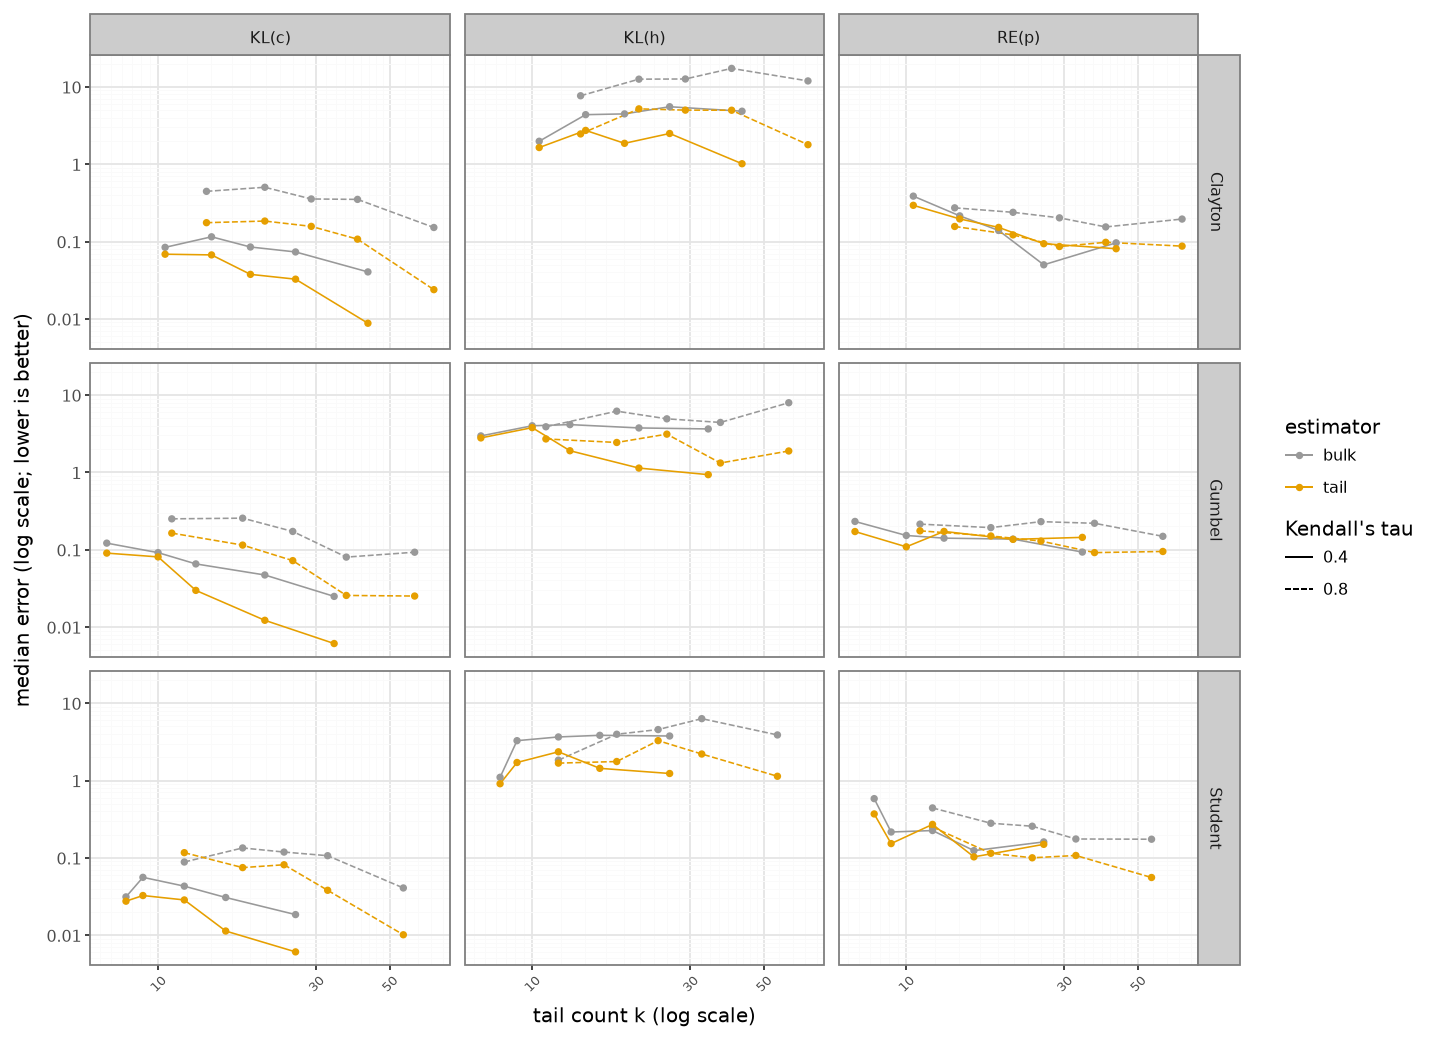
\includegraphics[width=\textwidth]{figures/sim_study.png}
  \caption{Median error of the bulk ($\hat c_B$) and tail ($\hat c_T$) estimators against the tail count $k$, over $20$ replications, for $n\in\{200,500,1000,2000,5000\}$ at Kendall's $\tau\in\{0.4,0.8\}$: generalized Kullback--Leibler divergence of the copula density $c$ and the tail-conditional density $h$, and relative error of the tail mass $p_n$ (columns). Both axes are logarithmic and lower is better. Gumbel is evaluated at the upper-right corner, Clayton and Student at the lower-left.}
  \label{fig:sim}
\end{figure}

\section{Asymptotic properties of the piece-together estimator}
TODO:
\begin{itemize}
  \item Prove consistency and asymptotic normality of $\hat c_T(u,v)$.
    \begin{itemize}
      \item Use the results of \citet{geenens2017probit} for the bulk estimator $\hat c_B$.
      \item Adapt to the fact that the tail estimator is based on a random number of observations.
    \end{itemize}
  \item Prove consistency and asymptotic normality of the raw piece-together estimator $\tilde c$.
  \item Prove consistency and asymptotic normality of the final piece-together estimator $\hat c$.
\end{itemize}

% \section{Reminders}

% Let $U=(U_1,\ldots,U_d)$ have copula $C$ and, when it exists, copula density
% \begin{align*}
% c(u)
% =
% \frac{\partial^d}{\partial u_1\cdots\partial u_d}C(u),
% \qquad u\in(0,1)^d.
% \end{align*}

% The lower tail copula is
% \begin{align*}
% \Lambda_L(x)
% =
% \lim_{q\downarrow 0}
% q^{-1} C(qx_1,\ldots,qx_d),
% \qquad x\in[0,\infty)^d.
% \end{align*}

% If $\Lambda_L$ is absolutely continuous, its lower tail copula density is
% \begin{align*}
% \lambda_L(x)
% =
% \frac{\partial^d}{\partial x_1\cdots\partial x_d}\Lambda_L(x),
% \qquad x\in(0,\infty)^d.
% \end{align*}

% Equivalently, in density form,
% \begin{align*}
%   q^{d-1} c(qx_1,\ldots,qx_d)
%   \to
%   \lambda_L(x),
% \end{align*}
% or
% \begin{align*}
%   c(qx_1,\ldots,qx_d)
%   \sim
%   q^{1-d}\lambda_L(x).
% \end{align*}

% For the upper tail, define the survival copula tail probability
% \begin{align*}
%   \bar C(u_1,\ldots,u_d)
%   =
%   \Pr(U_1>u_1,\ldots,U_d>u_d).
% \end{align*}

% Equivalently, in terms of the copula $C$,
% \begin{align*}
% \bar C(u)
% =
% \sum_{A\subseteq\{1,\ldots,d\}}
% (-1)^{|A|}
% C(v_A(u)),
% \end{align*}
% where
% \begin{align*}
% (v_A(u))_j
% =
% \begin{cases}
%   u_j, & j\in A,\\
%   1, & j\notin A.
% \end{cases}
% \end{align*}

% The upper tail copula is
% \begin{align*}
% \Lambda_U(x)
% =
% \lim_{q\downarrow 0}
% q^{-1}\bar C(1-qx_1,\ldots,1-qx_d),
% \qquad x\in[0,\infty)^d.
% \end{align*}

% If $\Lambda_U$ is absolutely continuous, its upper tail copula density is
% \begin{align*}
% \lambda_U(x)
% =
% \frac{\partial^d}{\partial x_1\cdots\partial x_d}\Lambda_U(x),
% \qquad x\in(0,\infty)^d.
% \end{align*}

% Equivalently, in density form,
% \begin{align*}
% q^{d-1} c(1-qx_1,\ldots,1-qx_d)
% \to
% \lambda_U(x),
% \end{align*}
% or
% \begin{align*}
% c(1-qx_1,\ldots,1-qx_d)
% \sim
% q^{1-d}\lambda_U(x).
% \end{align*}

% Thus, the tail copulas $\Lambda_L$ and $\Lambda_U$ are cumulative limit objects, while $\lambda_L$ and $\lambda_U$ are the corresponding local density limits obtained from the copula density $c$ near the lower and upper corners.

\bibliographystyle{apalike}
\bibliography{mybib}

\end{document}